\subsection{Performance of Osmotic Scaling and Load Balancing}
% 2 pages
With this experiment we want to provide baseline performance data for the osmotic scaling and scheduling method we propose. The goal is to show how our proposed solution operates without fine-tuning of parameters, or any other conditions. The experiment should also show how the osmotic scaling and scheduling of load balancers affects other parts of the serverless system, most notably the scaling decisions of regular functions.
\subsubsection{Setup}
Our experiment setup for these evaluations is once again based on the serverless edge computing simulator we also used for the initial evaluations. To stay consistent we used the same network topologies from the previous experiment that investigated the impact of load balancer scale on the system, meaning we assume clients to typically be connected via a mobile network, and compute resources to be distributed on the edge. The three topologies we tested are once again one scenario with a single city, one with three cities on the same continent, and one with three cities distributed across the globe. The cities chosen, along with the network latencies between them are the same as in the initial evaluation namely Chicago, New York, and Seattle for the nation-distibuted and New York, London, and Sydney for the globally-distributed experiment. The network latencies between them can be seen in tables \ref{tab:initial_nation_pings} and \ref{tab:initial_global_pings} respectively.

To stay consistent with the other experiments, and partially due to performance limitations, we once again tested each topology scenario with 25\gls{rps}, 50\gls{rps}, and 75\gls{rps}. As for the osmotic scaling and scheduling component, we set the pressure threshold for scaling up to 0.025 and the downscaling threshold to 0.03, which can roughly be read as the system requiring an expected \gls{trt} improvement of 2.5\% and 3\% to add or remove a load balancer instance on a given node. Bear in mind that this idea of required estimated performance improvement is a mental model to get a more intuitive understanding for the parameters, and is not equivalent to the actual implementation.

The last way in which the experiment setup differs from the previous experiments is that there is a function scheduling component active. While the other experiments purposefully set a fixed scale for each of the serverless functions in the system to avoid it as a confounding variable, these experiments use a dynamic function scaler to show how this type of load balancer scaling and scheduling affects the overall system.
In concrete terms, we set the simulator up to use a set rate of average requests per function replica.
The reasoning behind this choice is that OpenFaaS uses the same methodology as a default configuration, which we use as a stand-in example of serverless computing frameworks in general.
For the osmotic scaling and scheduling parameters we used 0.03 as a scale-up threshold and 0.05 as a scale-down threshold.

\subsubsection{Results}

\begin{table}[]
\begin{tabular}{lrrrrrr}
\hline
\textbf{Experiment}  & \textbf{\begin{tabular}[c]{@{}r@{}}LB\\ replicas\end{tabular}} & \textbf{\begin{tabular}[c]{@{}r@{}}Converged\\ Total \\ Function\\ Replicas\end{tabular}} & \textbf{\begin{tabular}[c]{@{}r@{}}Cross-City\\ Request\\ Share\end{tabular}} & \textbf{\begin{tabular}[c]{@{}r@{}}Mean\\ TRT\end{tabular}} & \textbf{\begin{tabular}[c]{@{}r@{}}Median\\ TRT\end{tabular}} & \textbf{\begin{tabular}[c]{@{}r@{}}Q90\\ TRT\end{tabular}} \\ \hline
25rps City LRT       & 6                                                              & 88                                                                                        & 0.0\%                                                                         & 121ms                                                       & 121ms                                                         & 157ms                                                      \\
25rps City Osmotic   & 24                                                             & 89                                                                                        & 0.0\%                                                                         & 117ms                                                       & 119ms                                                         & 149ms                                                      \\
25rps City RR        & 6                                                              & 90                                                                                        & 0.0\%                                                                         & 168ms                                                       & 136ms                                                         & 275ms                                                      \\ \hline
25rps Nation LRT     & 14                                                             & 89                                                                                        & 17.0\%                                                                        & 154ms                                                       & 131ms                                                         & 254ms                                                      \\
25rps Nation Osmotic & 3                                                              & 88                                                                                        & 32.5\%                                                                        & 224ms                                                       & 208ms                                                         & 386ms                                                      \\
25rps Nation RR      & 14                                                             & 90                                                                                        & 65.4\%                                                                        & 274ms                                                       & 266ms                                                         & 432ms                                                      \\ \hline
25rps Global LRT     & 14                                                             & 94                                                                                        & 0.4\%                                                                         & 142ms                                                       & 126ms                                                         & 210ms                                                      \\
25rps Global Osmotic & 5                                                              & 90                                                                                        & 1.7\%                                                                         & 152ms                                                       & 128ms                                                         & 224ms                                                      \\
25rps Global RR      & 14                                                             & 99                                                                                        & 65.4\%                                                                        & 501ms                                                       & 410ms                                                         & 937ms                                                      \\ \hline
50rps City LRT       & 6                                                              & 249                                                                                       & 0.0\%                                                                         & 127ms                                                       & 124ms                                                         & 177ms                                                      \\
50rps City Osmotic   & 13                                                             & 249                                                                                       & 0.0\%                                                                         & 123ms                                                       & 123ms                                                         & 164ms                                                      \\
50rps City RR        & 6                                                              & 249                                                                                       & 0.0\%                                                                         & 162ms                                                       & 141ms                                                         & 248ms                                                      \\ \hline
50rps Nation LRT     & 14                                                             & 179                                                                                       & 17.7\%                                                                        & 153ms                                                       & 129ms                                                         & 270ms                                                      \\
50rps Nation Osmotic & 5                                                              & 177                                                                                       & 24.3\%                                                                        & 165ms                                                       & 135ms                                                         & 283ms                                                      \\
50rps Nation RR      & 14                                                             & 181                                                                                       & 65.0\%                                                                        & 271ms                                                       & 264ms                                                         & 430ms                                                      \\ \hline
50rps Global LRT     & 14                                                             & 190                                                                                       & 1.2\%                                                                         & 147ms                                                       & 128ms                                                         & 213ms                                                      \\
50rps Global Osmotic & 4                                                              & 181                                                                                       & 3.8\%                                                                         & 159ms                                                       & 128ms                                                         & 238ms                                                      \\
50rps Global RR      & 14                                                             & 197                                                                                       & 65.1\%                                                                        & 494ms                                                       & 410ms                                                         & 922ms                                                      \\ \hline
75rps City LRT       & 6                                                              & 249                                                                                       & 0.0\%                                                                         & 127ms                                                       & 123ms                                                         & 175ms                                                      \\
75rps City Osmotic   & 14                                                             & 249                                                                                       & 0.0\%                                                                         & 122ms                                                       & 122ms                                                         & 162ms                                                      \\
75rps City RR        & 6                                                              & 249                                                                                       & 0.0\%                                                                         & 168ms                                                       & 140ms                                                         & 275ms                                                      \\ \hline
75rps Nation LRT     & 14                                                             & 269                                                                                       & 14.9\%                                                                        & 150ms                                                       & 129ms                                                         & 260ms                                                      \\
75rps Nation Osmotic & 5                                                              & 264                                                                                       & 24.1\%                                                                        & 169ms                                                       & 138ms                                                         & 287ms                                                      \\
75rps Nation RR      & 14                                                             & 269                                                                                       & 65.2\%                                                                        & 273ms                                                       & 269ms                                                         & 433ms                                                      \\ \hline
75rps Global LRT     & 14                                                             & 278                                                                                       & 0.1\%                                                                         & 141ms                                                       & 128ms                                                         & 214ms                                                      \\
75rps Global Osmotic & 5                                                              & 268                                                                                       & 1.9\%                                                                         & 152ms                                                       & 129ms                                                         & 223ms                                                      \\
75rps Global RR      & 14                                                             & 285                                                                                       & 65.2\%                                                                        & 497ms                                                       & 406ms                                                         & 928ms                                                      \\ \hline
\end{tabular}
\caption{Osmotic baseline evaluation results}
\label{tab:osmotic_base}
\end{table}

\begin{figure}
    \centering
    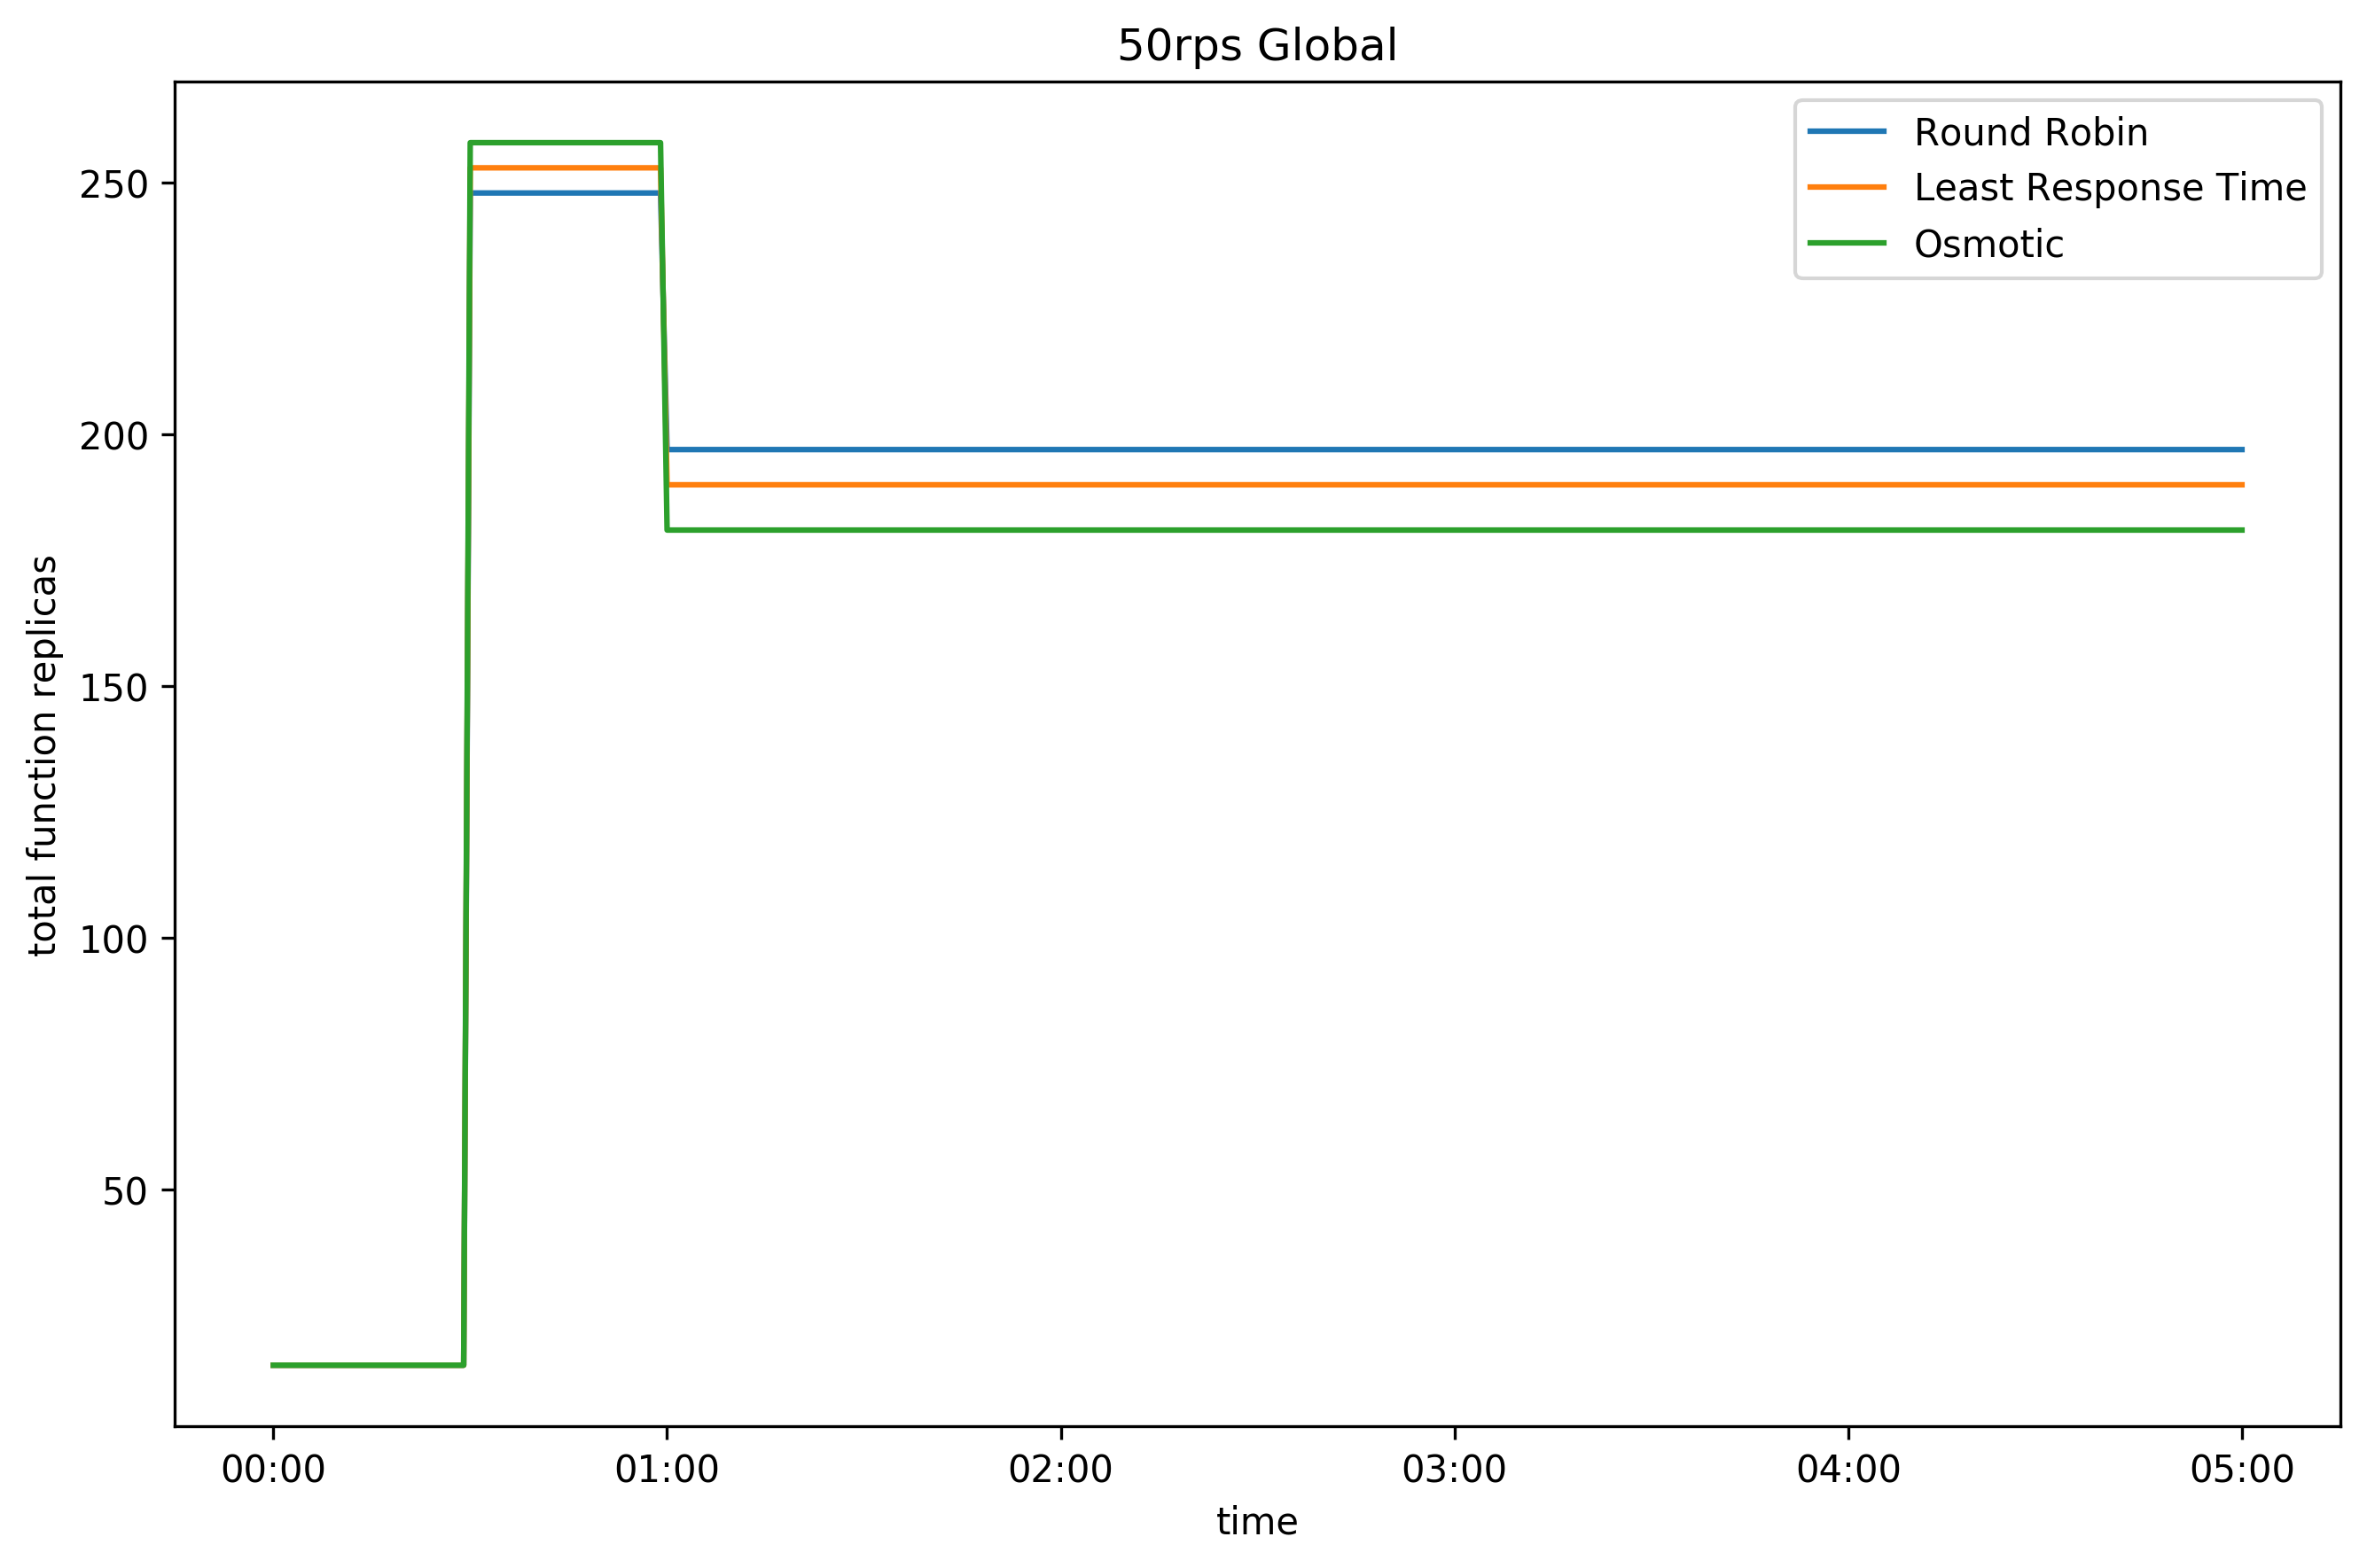
\includegraphics[width=12cm]{graphics/graphs/osmotic_base_function_scale_by_lb.png}
    \caption{Total scale of all functions for each load balancer scaling/schedulilng method}
    \label{fig:osmotic_fx_scale_by_scaling}
\end{figure}

Table \ref{tab:osmotic_base} shows the results of the experiment.
In terms of mean \gls{trt} performance the results of our proposed osmotic scaling and scheduling method are similar to those of the fixed scaling LRT reference setup, albeit between 1\% and 45\% worse with most scenarios only between 2\% and 8\% worse.
Differences between least response time static, and osmotic scaling are less pronounced in the median and 90th percentile \glspl{trt} as can also be seen in Table \ref{tab:osmotic_base}.
The statically scaled round robin load balancing is, as one would expect, significantly worse.
It does, however, give a good impression of the performance improvements possible based on our approach in a more complex and realistic deployment scenario than the initial evaluation.

We can also observe that in the city scenario the osmotic scaling and scheduling ends up deploying the more load balancer instances than the static scaling, but that for the nation- and globally-distributed network topology scenarios this patterns is reversed. There the osmotic scaler deploys only about a third of the replicas of the static scaling.

A similar pattern can be seen with regard to function scaling.
The osmotic scaling leads to between 1\% and 6\% fewer function replicas being deployed. Figure \ref{fig:osmotic_fx_scale_by_scaling} shows how the timing and frequency of scaling decisions are not different between the scaling methods, but osmotic scaling results in slightly fewer function replicas. 